\hypertarget{analyse}{%
\subsection{Analyse}\label{analyse}}

\hypertarget{intuxe9ruxeat-des-journaux-au-sujet-du-secret-bancaire}{%
\subsubsection{\texorpdfstring{Intérêt des journaux au sujet du
\emph{secret
bancaire}}{Intérêt des journaux au sujet du secret bancaire}}\label{intuxe9ruxeat-des-journaux-au-sujet-du-secret-bancaire}}

Le sujet du secret bancaire a suscité une centaine de premières pages au
sein des deux journaux de 1940 jusqu'à la fin des années 90. Ce chiffre
relativement petit nous permet de lire quelques premières pages pour
mieux mettre en contexte nos autres analyses.

De manière générale et excluant l'année 1984 de l'initiative populaire
au même sujet, le secret bancaire n'est pas un sujet très important dans
le corpus financier. Le sous-corpus ``secret bancaire'' ne constitue que
5\% des articles du corpus financier, qui lui-même ne contient qu'une
petite partie de tous les articles. Il est remarquable que dans le
sous-corpus la proportion d'articles qui proviennent d'agences de presse
est de dix pour-cent plus élevée que dans le corpus financier (29\% pour
le ``secret bancaire'', 18\% pour le financier). Cela pourrait être
justifié par l'hypothèse que le sujet a peu d'importance pour les
rédactions, qui n'utilisent souvent que des dépêches pour en parler.
Comme le montre le collage \ref{depeches}, les dépêches parlent surtout
de cas judiciaires et de petits scandales.

\begin{figure}
\centering
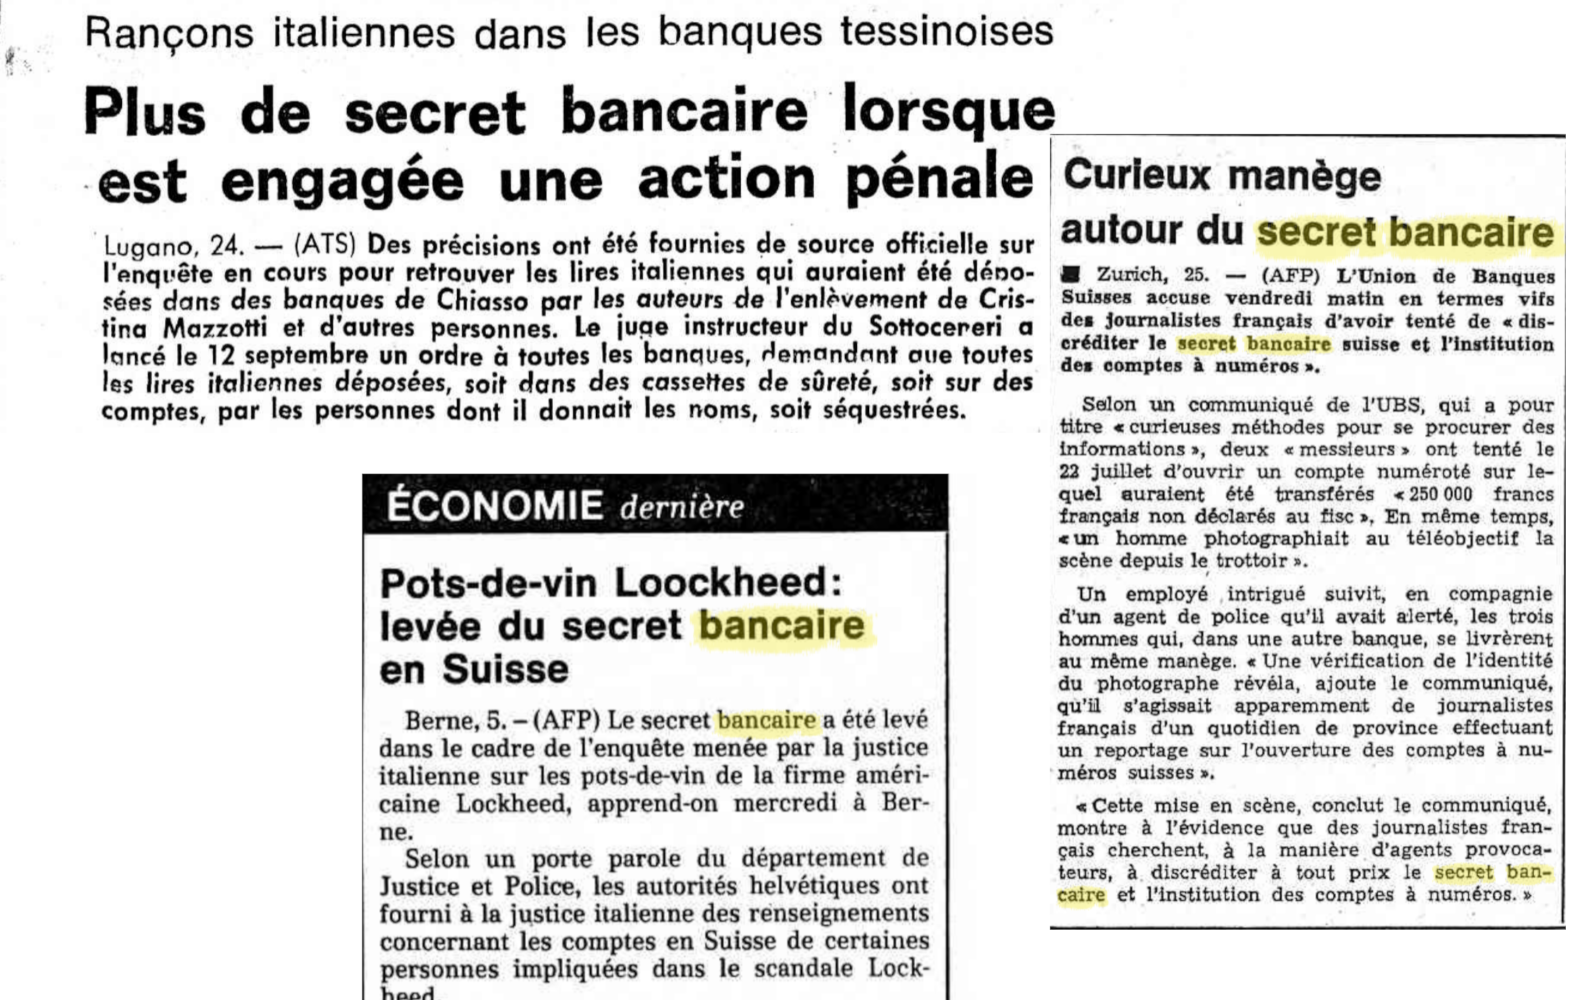
\includegraphics[width=0.9\textwidth,height=\textheight]{agencies_collage.png}
\caption{\label{depeches} Exemple de dépêches, suisses et étrangères.}
\end{figure}

Pour cerner l'origine de cet intérêt, nous comparons la fraction de
dépêches venant de l'étranger à celles de l'Agence télégraphique suisse
(ATS). La figure \ref{percentage1} montre comment cette fraction évolue
dans le sous-corpus au cours du temps. Nous trouvons deux périodes où
les dépêches étrangères ont une certaine présence: 1972 -- 1977 et 1986
-- 1992. Ce sont des périodes relativement calmes, où à l'intérieur de
la Suisse le sujet n'est pas d'actualité. Les dépêches dans le collage
\ref{depeches} représentent bien le type d'article sur des faits mineurs
apparaissant dans cette période calme.

\begin{figure}
\centering
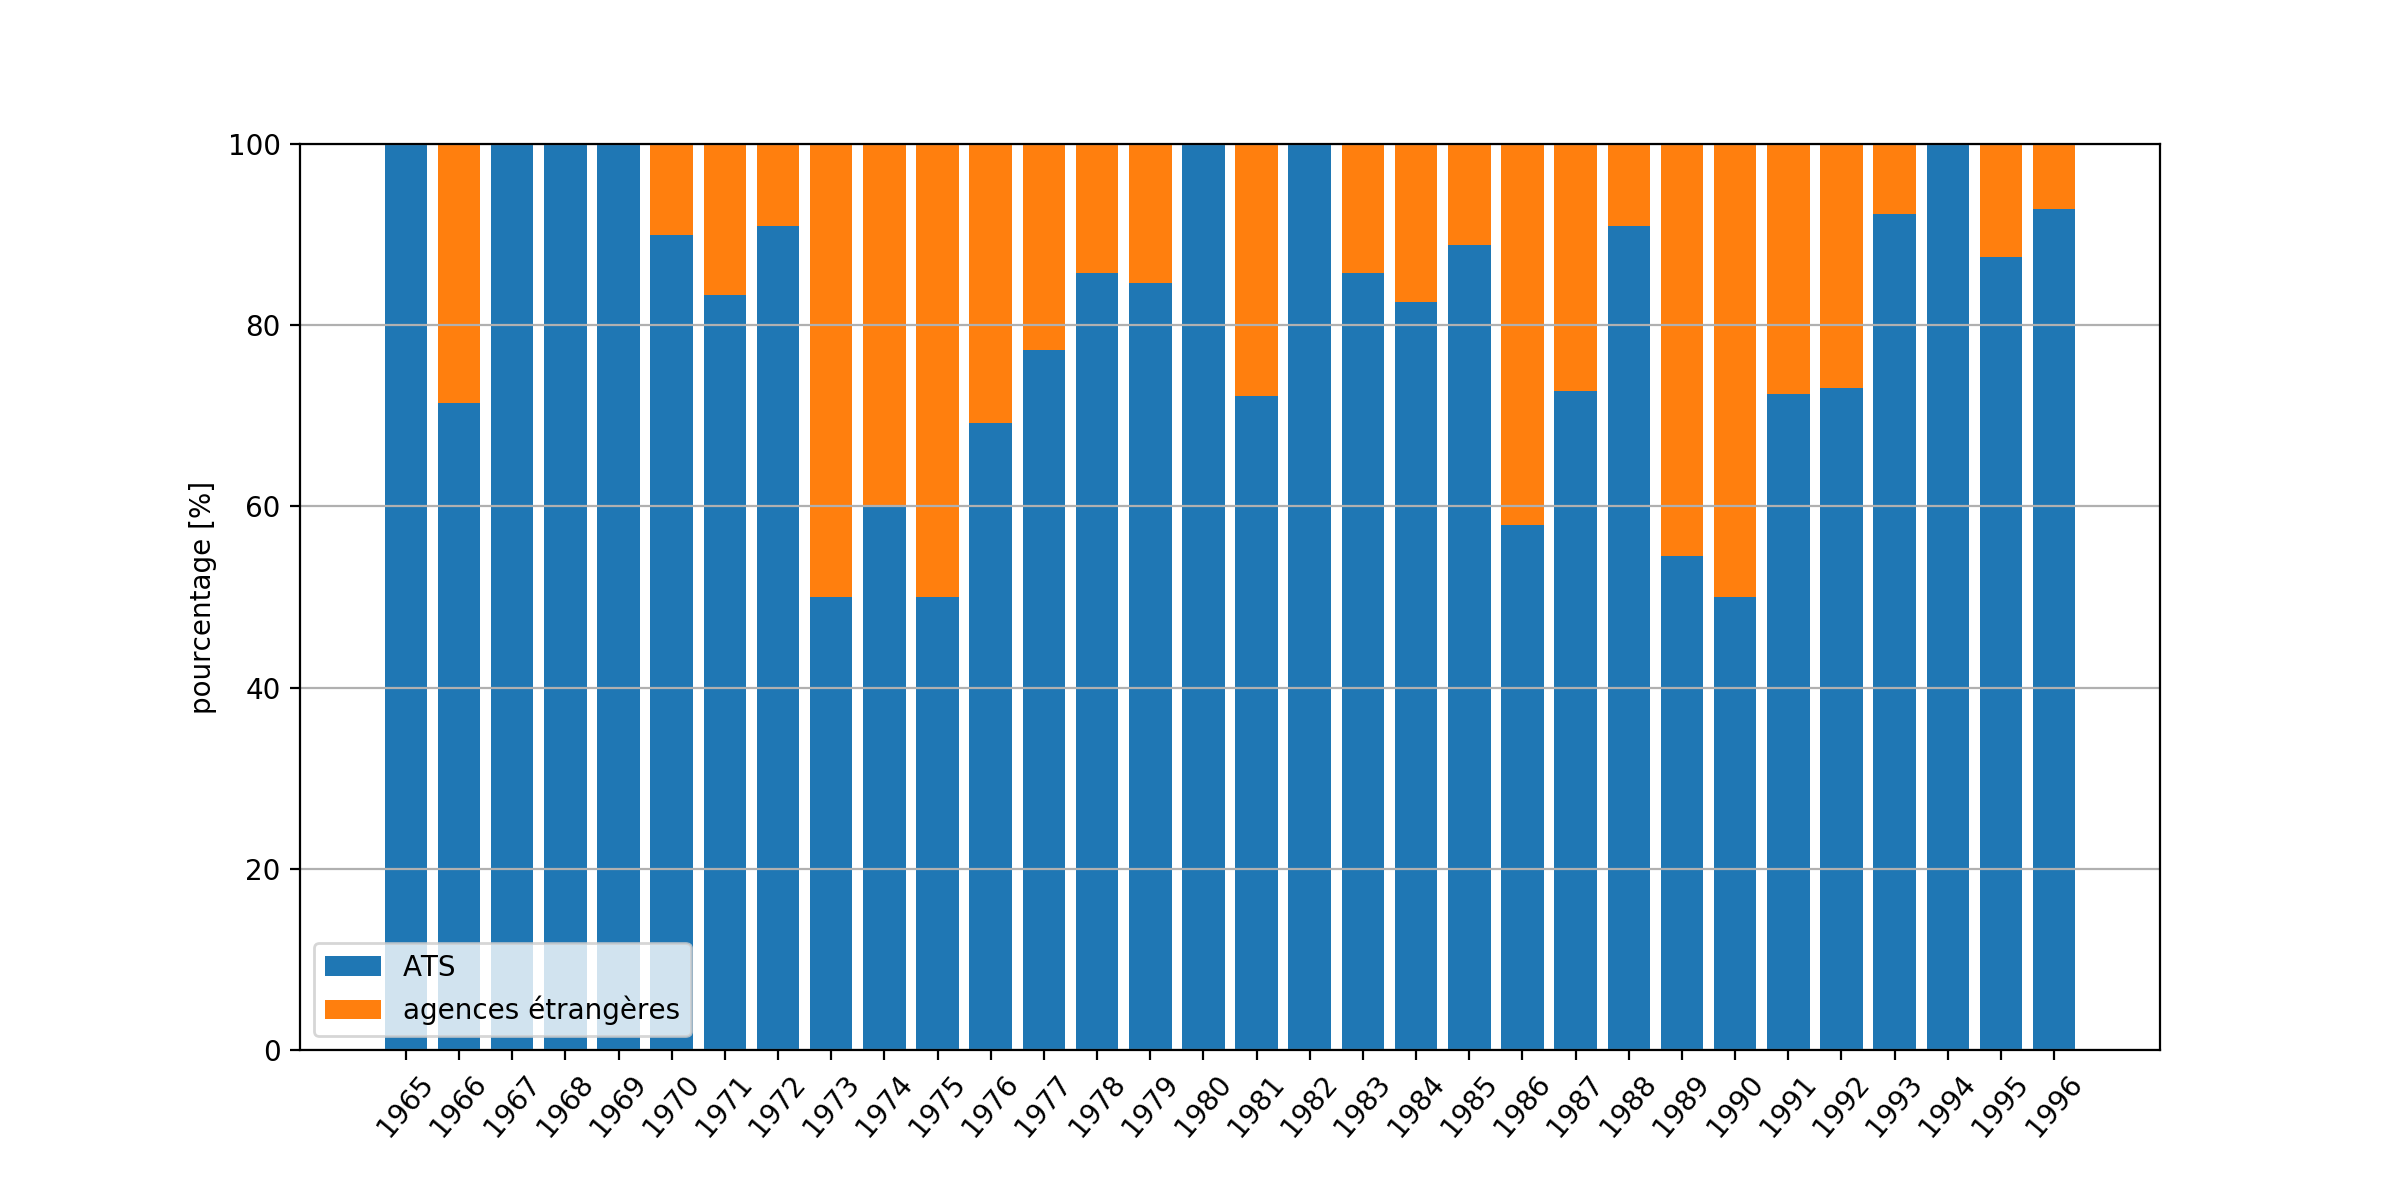
\includegraphics[width=0.9\textwidth,height=\textheight]{agency_percentage.png}
\caption{\label{percentage1} Distribution relative des articles
d'agences de presse étrangères pour le ``secret bancaire''.}
\end{figure}

La série temporelle du nombre d'articles par catégorie d'auteur (fig.
\ref{categorie}) met en évidence une nette chute de l'utilisation de
dépêches étrangères qui parlent du secret bancaire pendant exactement la
période avant la votation de 1984. Vue la forte orientation politique
des deux rédactions contre l'initiative, on peut supposer que les
articles d'agences étrangères qui ne concernent pas l'initiative sont
minimisés, pour ne pas détourner l'attention des lecteurs.

\begin{figure}
\centering
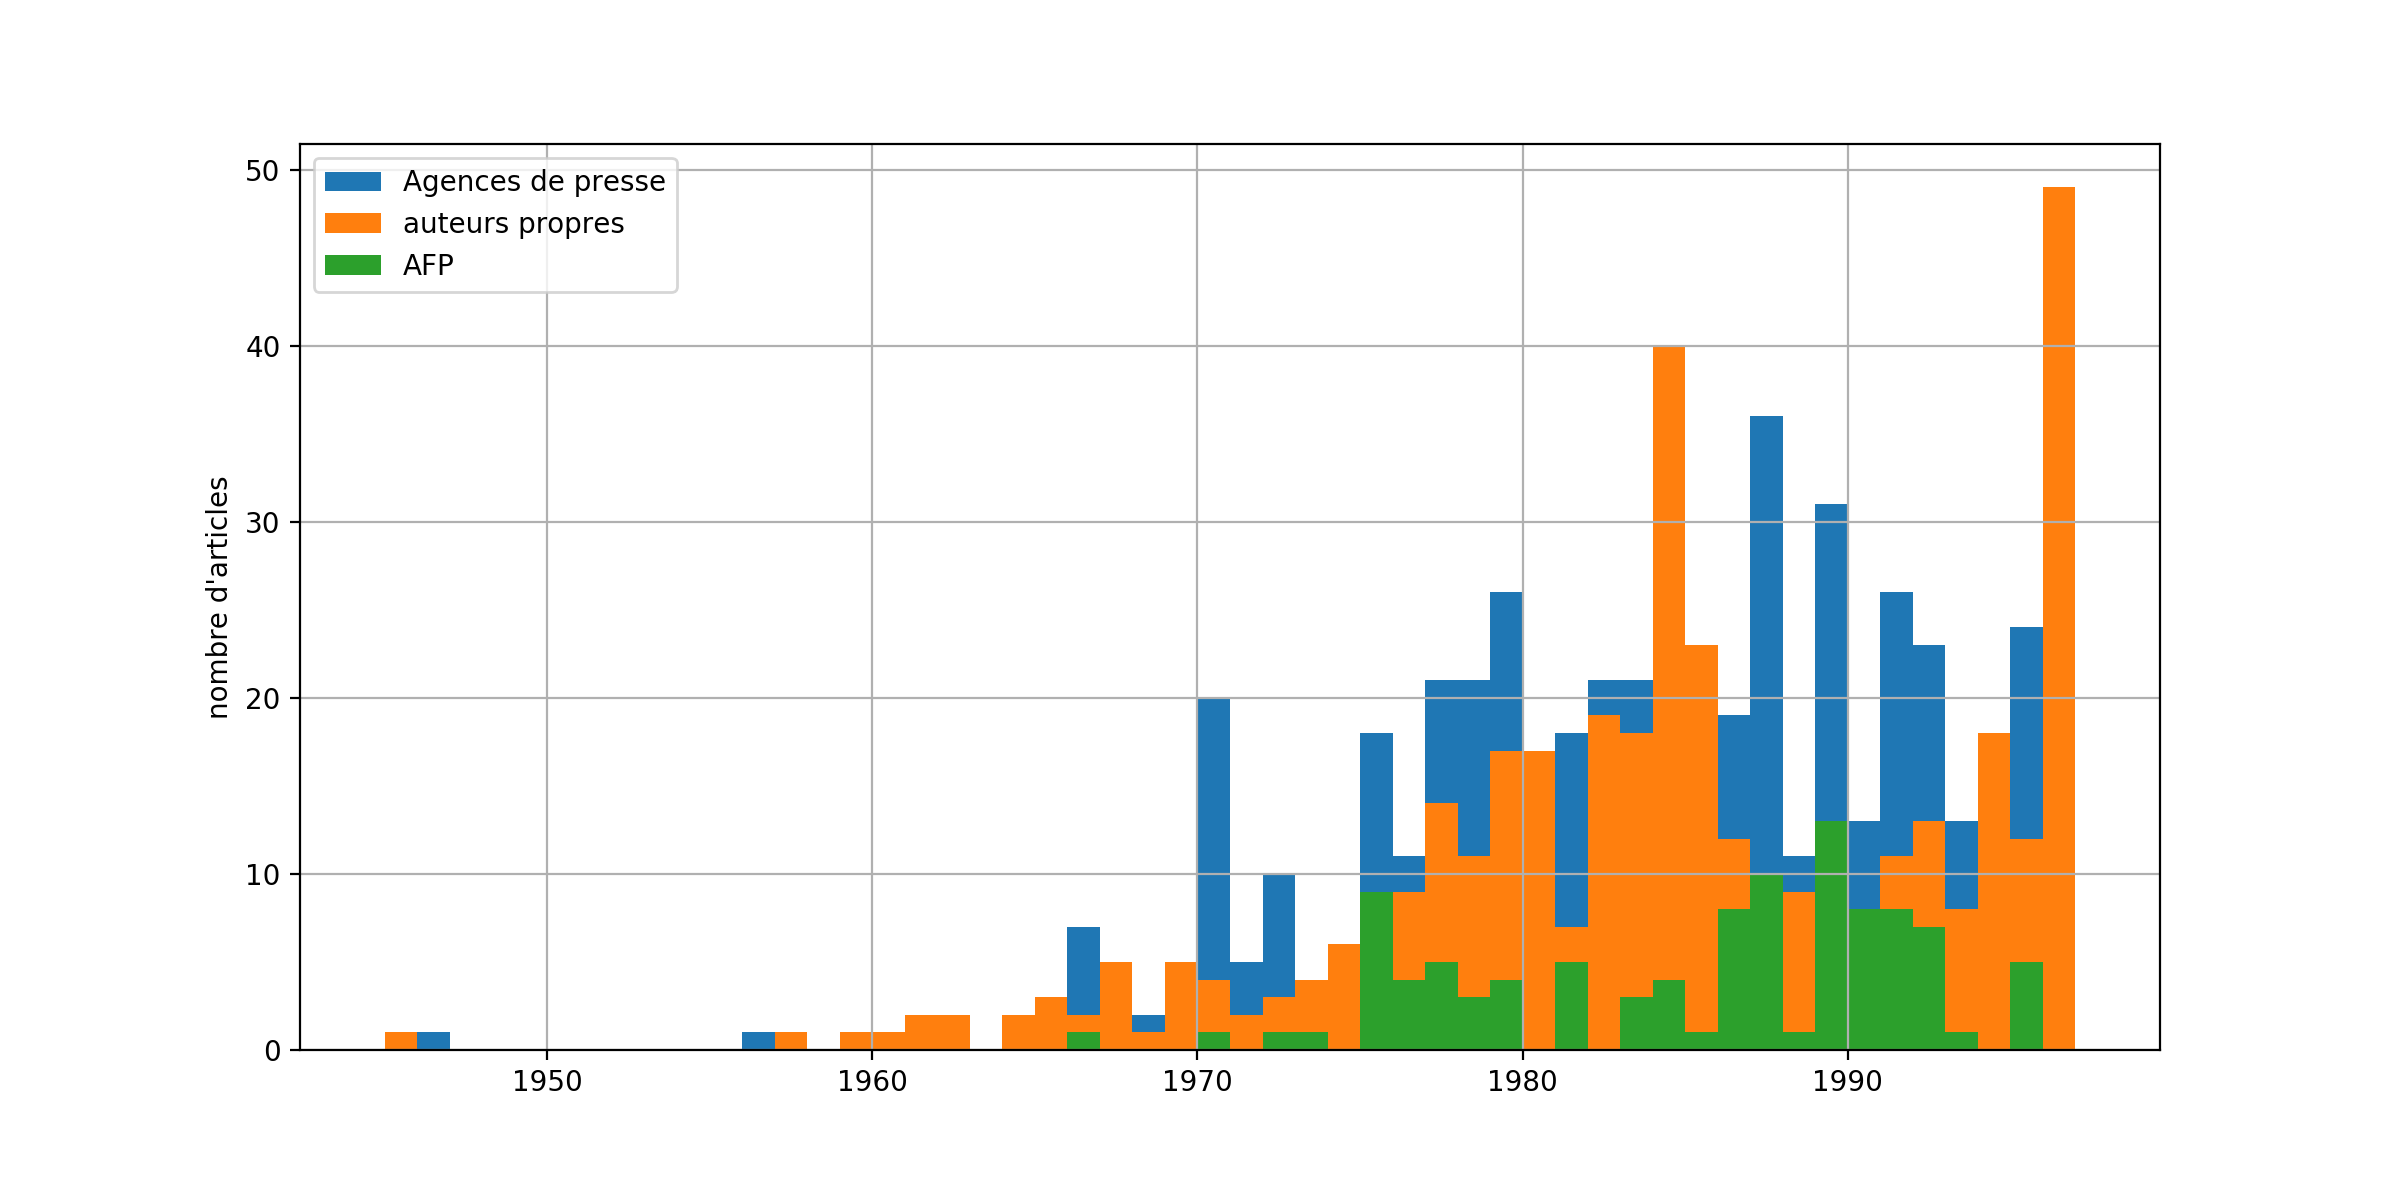
\includegraphics[width=0.9\textwidth,height=\textheight]{authors_agency_count.png}
\caption{\label{categorie} Nombre d'articles par catégorie d'auteur au
cour du temps.}
\end{figure}

Par la lecture des premières pages, nous trouvons le ensemble suivant de
périodes principales dans l'histoire du secret bancaire:

\begin{itemize}
\item
  1940--45: Le secret bancaire est menacé de l'intérieur par le
  gouvernement, à cause de l'économie de guerre, et de l'extérieur par
  les futures nations unies, qui désirent l'entraide judiciaire et
  fiscale.
\item
  1946--65: Période de calme où aucune attaque importante n'est montée
  contre le secret bancaire. Quelques frictions avec la France se
  résolvent en une impasse.
\item
  1966--70: Tensions et efforts diplomatiques avec les États-Unis, qui
  critiquent durement le secret bancaire qui leur empêche d'enquêter
  efficacement la criminalité organisée. Cela se résout avec des accords
  bilatéraux qui concèdent très peu à la justice américaine.
\item
  1975--84: Tumultes intérieurs vis au secret bancaire. L'économie en
  récession et la force du Franc Suisse dans les marchés de devises
  portent les milieux politiques socialistes à attaquer le secret
  bancaire comme responsable. Le débat intérieur continue jusqu'en 1984,
  quand l'initiative socialiste contre le secret bancaire est repoussée.
\item
  1987--89: Pressions américaines poussent la Suisse à approuver la
  levée du secret bancaire dans le cas de manipulation des marchés
  (\emph{insider trading}), un délit qui n'était pas persécuté en Suisse
  jusqu'alors.
\item
  1996--suite: Affaire des fonds juifs en déshérence. Le conseil
  national vote à l'unanimité pour la levée du secret bancaire pour la
  commission Bergier.
\end{itemize}

La tonalité du discours dans les deux journaux au cours de ces périodes
est surtout intéressante. Dans la première période, le ton est positif
et tranquille. En 1975, le ton change rapidement: des articles écrits
par Marian Stepcinsky, Jean-Luc Lederrey, et par le futur politicien
libéral Jacques-Simon Eggly gagnent souvent la première page. Ces
articles sont des pièces d'opinion, souvent virulentes, où les avantages
du secret bancaire sont rappelés. Contrairement aux périodes
précédentes, où ces avantages ont été considérés trop évidents pour les
souligner. Ces articles d'opinion forment une véritable propagande en
faveur du secret bancaire et contre les socialistes, et donnent de
précises indications de vote dans le mois avant l'initiative.

\begin{figure}
\centering
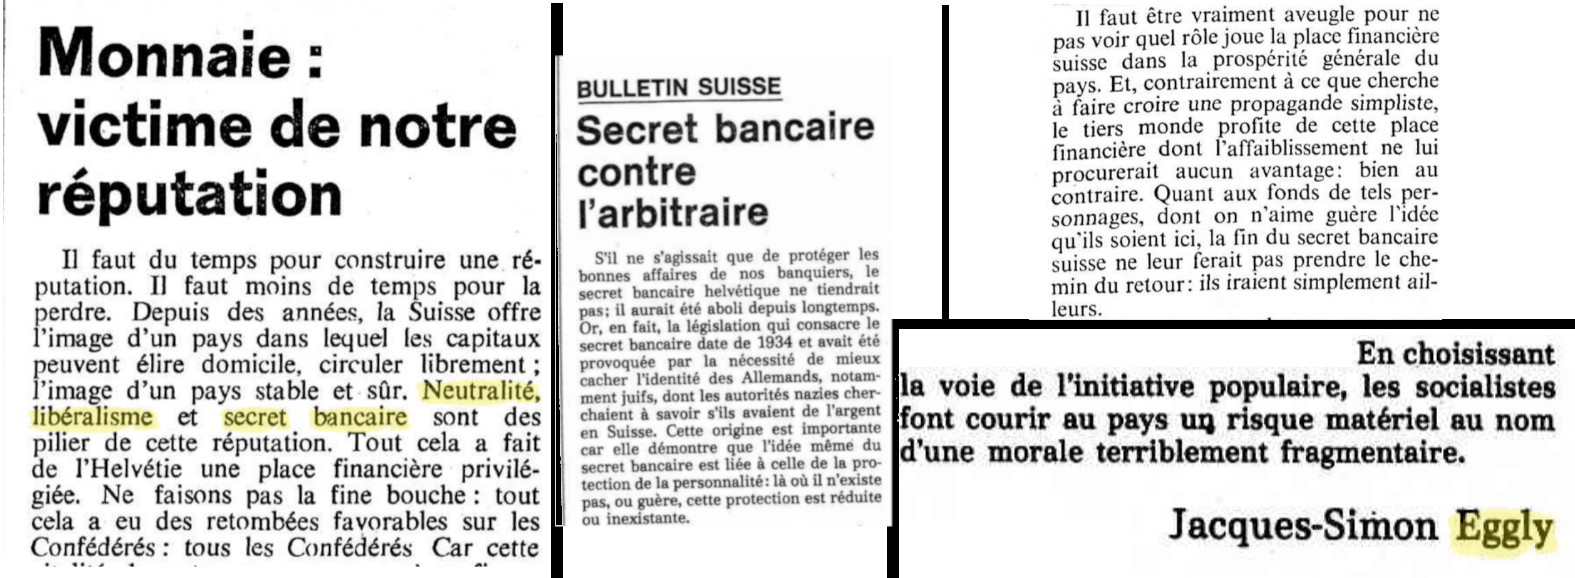
\includegraphics[width=0.9\textwidth,height=\textheight]{propaganda_collage.png}
\caption{\label{propagande} Exemple d'articles partisans apparus dans la
période de l'initiative.}
\end{figure}

La tonalité des articles redevient enfin plus descriptive et
s'assouplie, après que l'initiative soit rejetée. Les lois sur la
manipulation des marchés et la commission Bergier ne sont pas perçues
comme menace essentielles à la stabilité de la place financière.

\hypertarget{comparaison-des-deux-journaux}{%
\subsubsection{Comparaison des deux
journaux}\label{comparaison-des-deux-journaux}}

En isolant les articles contenant ``secret bancaire'', nous avons
auparavant isolé les articles en différents groupes avec la méthode de
Reinert. La première chose que nous remarquons est qu'entre les deux
journaux nous obtenons des groupes différents. Afin de mieux comprendre
comment les articles sont classés, nous avons aussi effectué des
Chi²-tests sur des mots-clés. Par exemple dans le \emph{Journal de
Genève}, nous pouvons voir que le terme ``UBS'' va éloigner l'article du
groupe contenant les termes plus proches du sujet, comme ``secret'',
``convention'', ``droit'' ou ``judiciaire'' que l'on voit dans la
première classe du dendrogramme (voir partie méthodologie). Cela pousse
l'article fortement vers le groupe trois qui contient des termes assez
descriptifs (sur les intérêts et les devises).

\begin{figure}
\centering
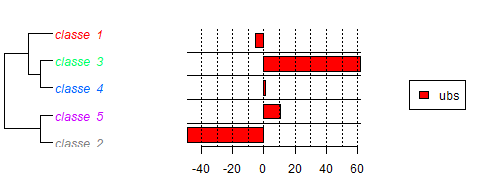
\includegraphics[width=0.9\textwidth,height=\textheight]{chiubs.png}
\caption{Chi²-Test du terme ``UBS'' dans le \emph{JDG}.}
\end{figure}

D'autres tests similaires pointent vers d'autres divisions, ou les
articles utilisants des termes juridiques et/ou techniques précis (comme
``bancaire'', ``fraude'', ``autorité'') vont concentrer les articles
dans une même classe. Mais nous voyons aussi que les termes qui ramènent
au nom des banques sont dissociés des groupes parlant de l'actualité du
secret bancaire.

Du côté de la \emph{GDL}, nous trouvons six groupes. Là ou le \emph{JDG}
semble avoir des classes qui sont basées sur des sujets différents
(économie, affaires judiciaires, légal), dans la \emph{GDL} il semble
que les événements marquants de la période génèrent plus d'attention.
Car, on retrouve une classe avec des mots rappelant des affaires
judiciaires. Dans cette classe on retrouve des termes tels que
``renseignement'', ``tribunal'', ``violer''\ldots{} Cela semble indiquer
que les différents scandales entourant le secret bancaire sont perçus
comme plus importants dans la \emph{GDL} que le \emph{JDG}. Cependant,
ici comme dans le \emph{JDG} le nom des banques suisses apparaît plutôt
dans le groupe d'articles référençant des termes financiers plus
généraux: la classe 3, qui est très similaire à la classe 3 dans
l'analyse du \emph{JDG} (avec les noms de devises et des quantités).

\begin{figure}
\centering
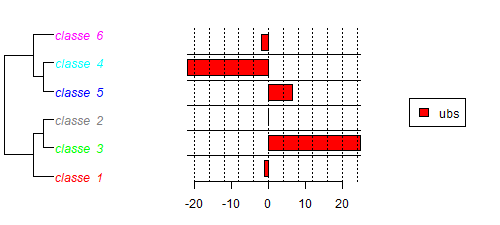
\includegraphics[width=0.9\textwidth,height=\textheight]{ubs_chisquare_gdl.png}
\caption{Chi²-Test du terme ``UBS'' dans la \emph{GDL}.}
\end{figure}

Tout ceci semble indiquer que, même si l'emphase apportée aux différents
événements entourant le secret bancaire est différente entre les deux
journaux, les deux semblent aussi dissocier les banques du sujet même du
secret bancaire.

\hypertarget{conclusions}{%
\subsubsection{Conclusions}\label{conclusions}}

Cette analyse du sujet évidence clairement l'adhésion des deux
rédactions à la politique libérale. L'absence de dépêches étrangères,
surtout centrées sur les scandales, pendant la période de l'initiative
peut être considérée comme une forte indication du rôle politique des
deux journaux.

L'analyse linguistique nous montre que la \emph{GDL} donne plus
d'importance aux affaires concrètes et le \emph{JDG} plus au coté
abstrait législatif, bien que aucun des deux journaux ne pointe jamais
du doigt. Dans les deux journaux, le secret bancaire est abordé dans un
contexte politique plutôt que financier, en défendant ces principes à la
base plutôt qu'en montrant les inconvénients qu'il cause aux fiscs et
aux investigateurs internationaux.
